
% Copyright (c) 2015 - 2020 Mario Mlačak, mmlacak@gmail.com
% Licensed and published as Public Domain work.

% Miranda's veil chapter ==============================================
\chapter*{Miranda's veil}
\addcontentsline{toc}{chapter}{Miranda's veil}

\begin{flushright}
\parbox{0.8\textwidth}{
\emph{Under all that we think, lives all we believe, like the ultimate veil of our spirits. \\
\hspace*{\fill}{\textperiodcentered \textperiodcentered \textperiodcentered \hspace*{0.2em} Antonio Machado} } }
\end{flushright}

\noindent
Miranda's veil is chess variant which is played on 16 x 16 board, with
white and dark violet fields and light magenta and indigo pieces. In
algebraic notation, columns are enumerated from 'a' to 'p', and rows
are enumerated from '1' to '16'. A new piece is introduced, Wave.

\clearpage % ..........................................................
% Wave ****************************************************************

\section*{Wave}
\addcontentsline{toc}{section}{Wave}

\vspace*{-1.0ex}
\noindent
\begin{wrapfigure}[12]{l}{0.4\textwidth}
\centering
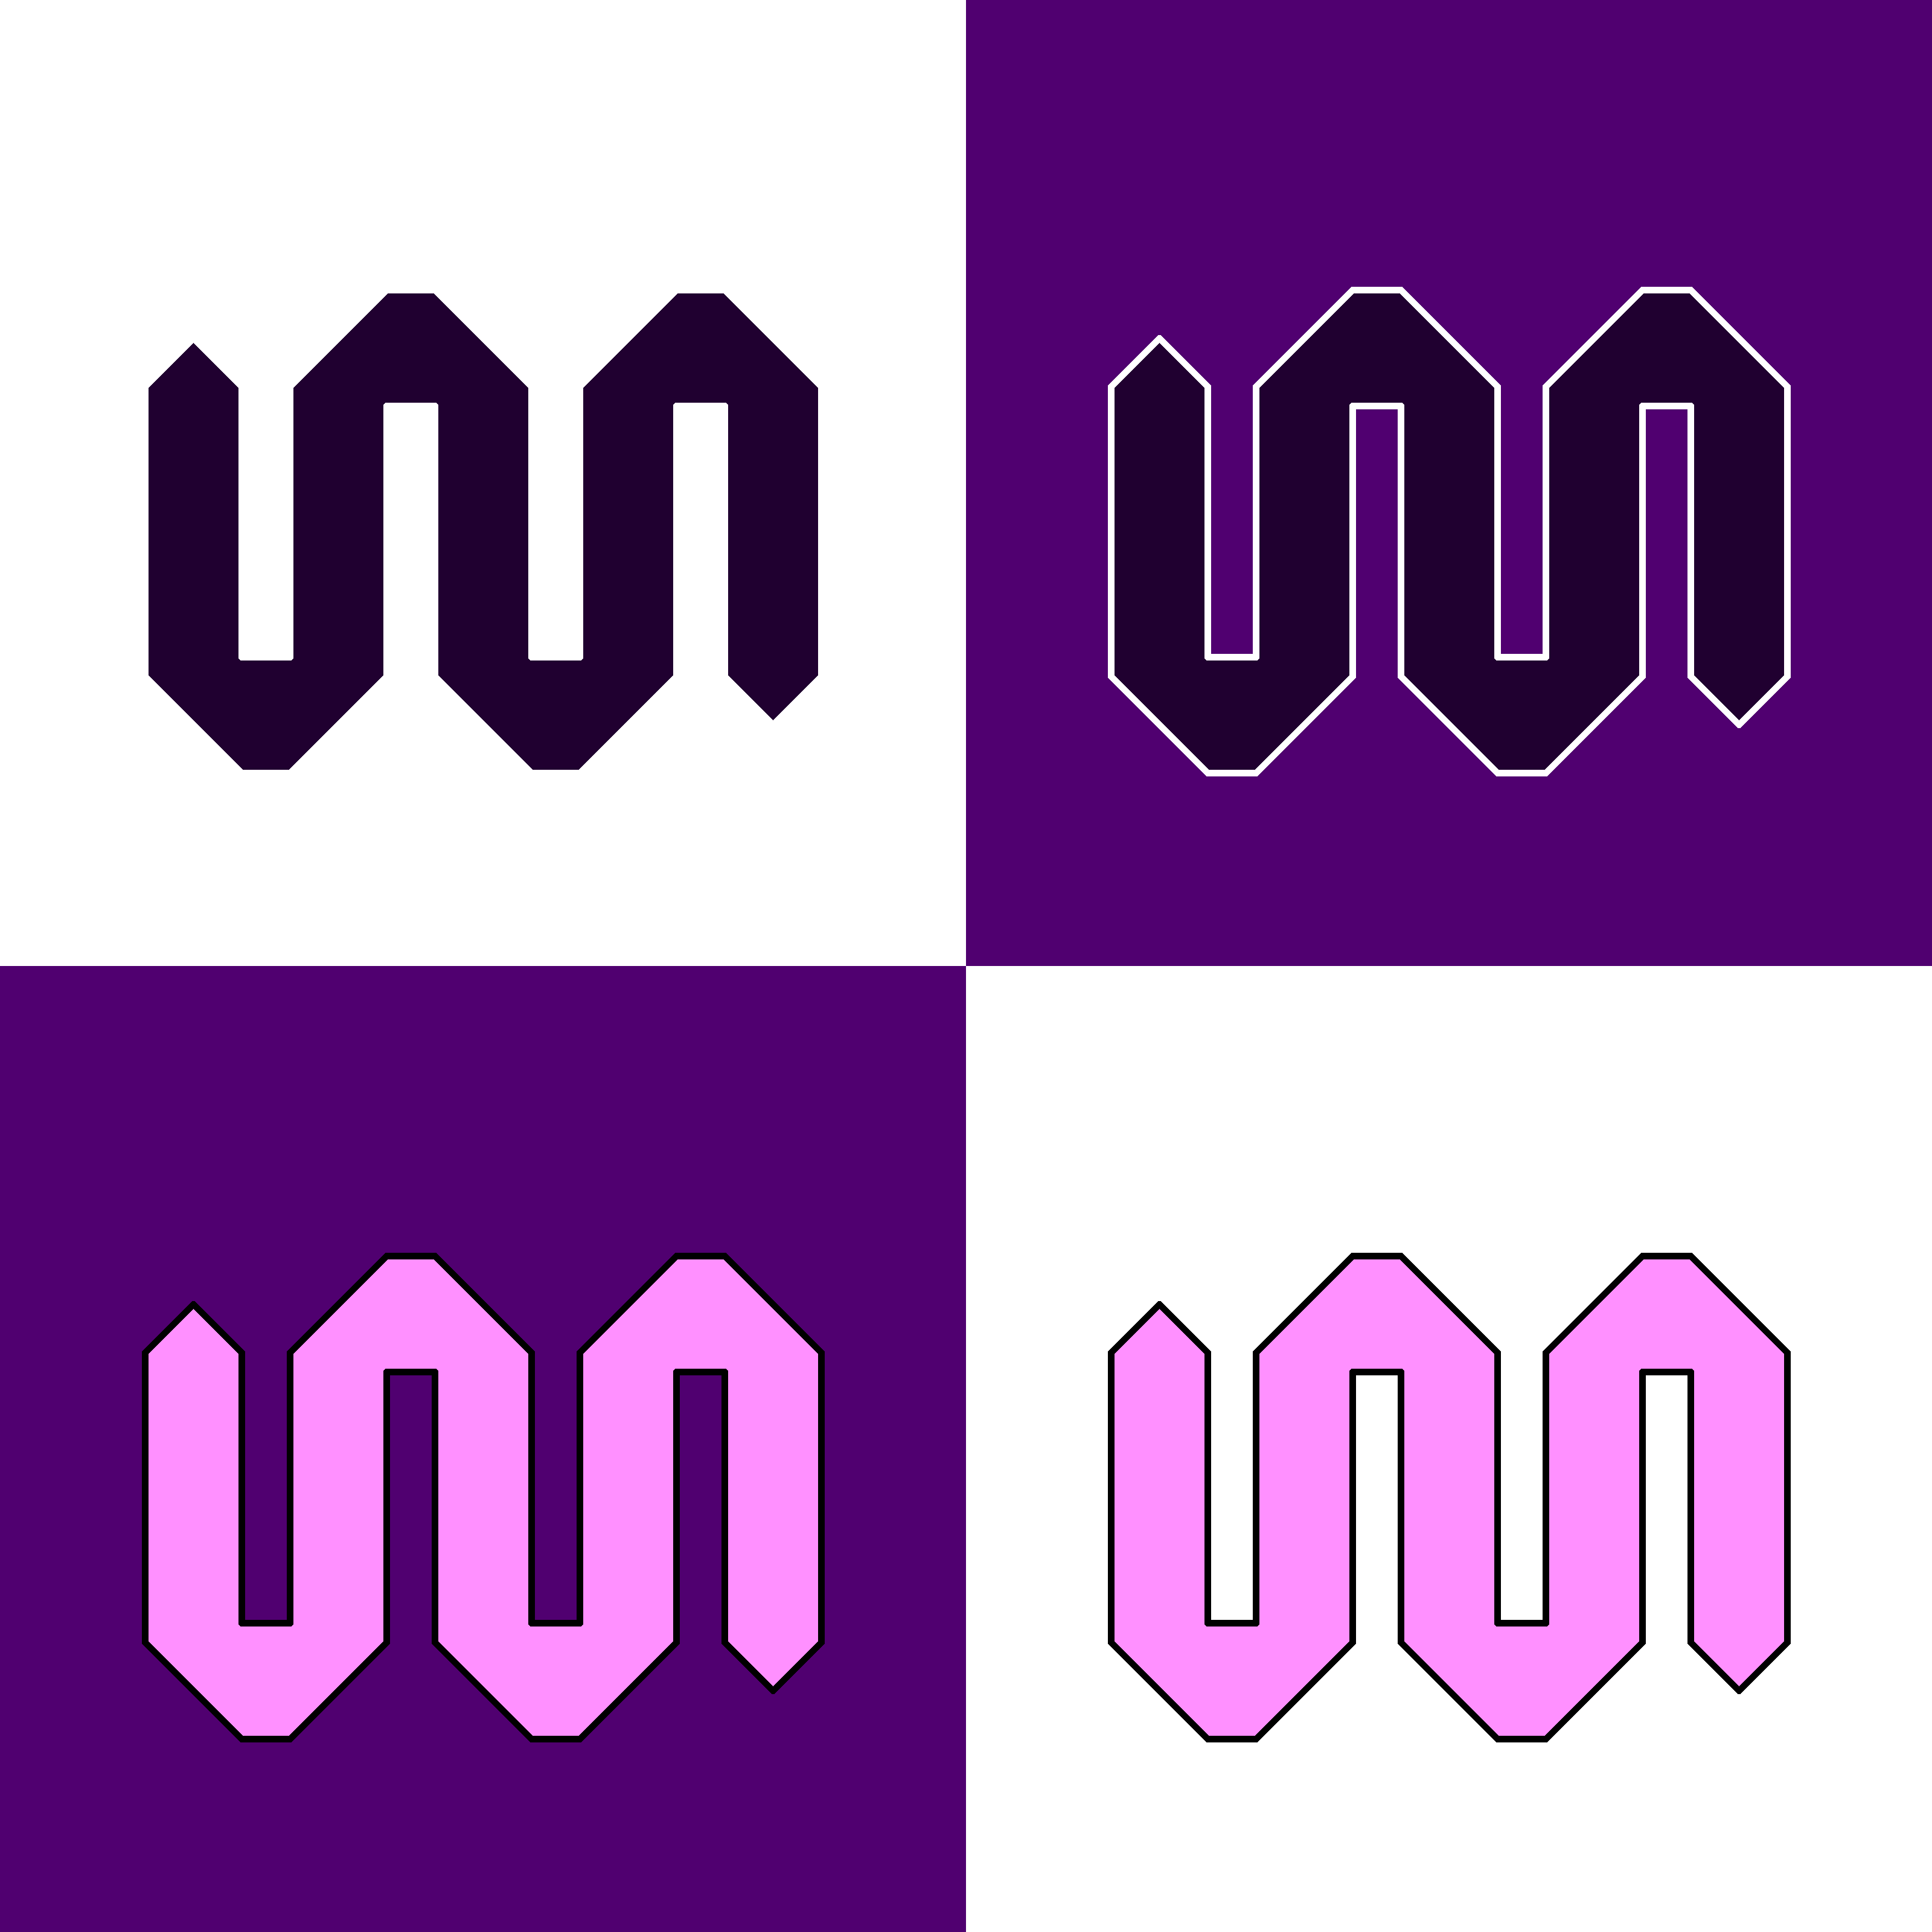
\includegraphics[width=0.4\textwidth, keepaspectratio=true]{pieces/10_wave.png}
\caption{Wave}
\label{fig:10_wave}
\end{wrapfigure}
Wave is passive piece, it has to be activated before it can move. Activation
is done in the same way as with Pyramid. Own piece has to capture field at
which Wave is located before Wave can move.

Wave can be activated even if activating piece has no momentum. Wave does not use
received momentum for moving, and isn't limited by it. Wave can move even if it
has no momentum. Wave can move past (pass "through") any piece, as if it isn't there.

After activation Wave moves like activating piece, over piece's step- or capture-
fields, depending where it was activated. Wave can make multiple steps, in the
same way activating piece does, even if activating piece can make only one. Note,
Wave can choose direction on the first 1 or 2 step(s), which cannot be changed
later. Wave can step outside of a chessboard, and only has to end its ply on a
board. For details see
\hyperref[sec:Appendix/Movement of Wave]{Movement of Wave}.

Wave cannot capture any piece. Thus, Wave cannot check nor checkmate opponent's
King.

Wave can activate any own piece, except King, if it has momentum. Wave can
also activate other Wave, own or opponent's, even if it has no momentum. In
all cases, Wave transfers all received momentum to activated piece.

In algebraic notation symbol for Wave is 'W'.

\clearpage % ..........................................................
% Activation ----------------------------------------------------------

\subsection*{Activation}
\addcontentsline{toc}{subsection}{Activation}

\vspace*{-2.0ex}
\noindent
% \begin{figure}[t]
\begin{figure}[h]
\includegraphics[width=1.0\textwidth, keepaspectratio=true]{examples/10_mv/scn_mv_01_move_wave_init.png}
\caption{Wave activation}
\label{fig:scn_mv_01_move_wave_init}
% \centering
\end{figure}

Above, after activation Wave could move the same way Knight does, over multiple
step-fields. Once Wave starts moving in a chosen direction, it cannot be changed.
So, in this case Wave would move as Pegasus does. Wave does not spend received
momentum while moving, and would transfer it entirely to any piece it activates.

\clearpage % ..........................................................

\noindent
% \begin{figure}[t]
\begin{figure}[h]
\includegraphics[width=1.0\textwidth, keepaspectratio=true]{examples/10_mv/scn_mv_02_move_wave_activated.png}
\caption{Wave activated}
\label{fig:scn_mv_02_move_wave_activated}
% \centering
\end{figure}

Wave can move unhindered by any piece, even on step-fields (green arrows). Wave
can also activate pieces (blue arrows) obscured by others, for instance light
Pyramid which is out of reach for regular Pegasus. Wave cannot activate Kings nor
opponent's pieces (red arrows), except dark Wave. \\
Again, Wave cannot change direction of movement after first step. For instance,
upon reaching step-field 5, it cannot change direction to 5c, or any other
greyed-out arrow.

\clearpage % ..........................................................

\noindent
% \begin{figure}[t]
\begin{figure}[h]
\includegraphics[width=1.0\textwidth, keepaspectratio=true]{examples/10_mv/scn_mv_03_move_wave_finished.png}
\caption{Wave finished}
\label{fig:scn_mv_03_move_wave_finished}
% \centering
\end{figure}

Greyed-out arrows show steps Wave have taken in its ply. Activated Bishop
now continues the move according to own rules of movement, i.e. diagonally.
Note that it's restricted by momentum received, and thus can make only one
step, i.e. can move for only one step.

\clearpage % ..........................................................

\subsubsection*{No momentum}
\addcontentsline{toc}{subsubsection}{No momentum}

\vspace*{-3.0ex}
\noindent
% \begin{figure}[t]
\begin{figure}[h]
\includegraphics[width=1.0\textwidth, keepaspectratio=true]{examples/10_mv/scn_mv_04_wave_no_momentum_no_activating.png}
\caption{No momentum}
\label{fig:scn_mv_04_wave_no_momentum_no_activating}
% \centering
\end{figure}

Wave can be activated with no momentum, if so it can activate only other Waves, but
cannot activate ordinary (non-Wave) pieces. Here, one momentum originating from Bishop
has been already spent by Knight, so Wave B is activated with no momentum, and so it
cannot activate Pawn. Wave B can pass-by Pawn, and activate dark Wave, also with no
momentum.

\clearpage % ..........................................................

\subsubsection*{Piece blocked}
\addcontentsline{toc}{subsubsection}{Piece blocked}

\vspace*{-3.0ex}
\noindent
% \begin{figure}[t]
\begin{figure}[h]
\includegraphics[width=1.0\textwidth, keepaspectratio=true]{examples/10_mv/scn_mv_05_wave_no_activating_blocked_piece.png}
\caption{Piece blocked}
\label{fig:scn_mv_05_wave_no_activating_blocked_piece}
% \centering
\end{figure}

Wave cannot activate blocked pieces, even if it has momentum. Here, Pawn is blocked
from moving forward by own Bishop, and there are no opponent's pieces on its'
diagonal capture-fields. So, Wave cannot activate Pawn, even though it has one
momentum received from Knight.

\clearpage % ..........................................................

\subsubsection*{Wave blocked}
\addcontentsline{toc}{subsubsection}{Wave blocked}

\vspace*{-3.0ex}
\noindent
% \begin{figure}[t]
\begin{figure}[h]
\includegraphics[width=1.0\textwidth, keepaspectratio=true]{examples/10_mv/scn_mv_06_wave_blocked_init.png}
\caption{Activating Wave}
\label{fig:scn_mv_06_wave_blocked_init}
% \centering
\end{figure}

Wave cannot activate opponent's pieces, except for Waves. Activated Wave which movement
is completely blocked is oblationed, i.e. is removed from chessboard as if captured by
opponent.

Here, dark Wave B is about to be activated with one momentum.

\clearpage % ..........................................................

\vspace*{-5.0ex}
\noindent
% \begin{figure}[t]
\begin{figure}[h]
\includegraphics[width=1.0\textwidth, keepaspectratio=true]{examples/10_mv/scn_mv_07_wave_blocked_end.png}
\caption{Activated Wave blocked}
\label{fig:scn_mv_07_wave_blocked_end}
% \centering
\end{figure}

Here, dark Wave B is activated without committing its movement yet (it's "in-the-air").
All accessible step-fields are blocked by opponent's light pieces, which cannot be
activated by dark Wave, even though it has one momentum.
Note, Wave (just like any other piece) has to move away from its starting position,
it cannot stay and re-activate piece that has activated it (here, light Wave 2).
Thus, dark Wave B is oblationed, i.e. removed from chessboard.

% ---------------------------------------------------------- Activation
\clearpage % ..........................................................
% Cascading Waves -----------------------------------------------------

\subsection*{Cascading Waves}
\addcontentsline{toc}{subsection}{Cascading Waves}

\noindent
\begin{wrapfigure}[13]{l}{0.5625\textwidth}
\centering
\includegraphics[width=0.5625\textwidth, keepaspectratio=true]{examples/10_mv/scn_mv_08_cascading_rook.png}
\caption{Rook starting cascade}
\label{fig:scn_mv_08_cascading_rook}
\end{wrapfigure}
Cascading Waves refers to a move in which two or more Waves have been displaced.
For example, Wave can activate another Wave. Wave can also activate active
piece (or Pyramid), which can then activate another Wave.

On the left, Rook is about to activate Wave 1, giving it momentum of 4.

\vspace*{0.05\textheight}
\noindent
\begin{wrapfigure}[12]{r}{0.5625\textwidth}
\centering
\includegraphics[width=0.5625\textwidth, keepaspectratio=true]{examples/10_mv/scn_mv_09_cascading_wave_1.png}
\caption{Wave 1 cascading}
\label{fig:scn_mv_09_cascading_wave_1}
\end{wrapfigure}
Activated Wave 1 inherits rules of movement from activating piece, and so now
moves as Rook would. It's not obstructed with any piece in its way, nor it's
limited by received momentum, i.e. it can move further than just 4 fields away.
Wave 1 can also activate Wave 2.

\clearpage % ..........................................................

\noindent
\begin{wrapfigure}[13]{l}{0.5625\textwidth}
\centering
\includegraphics[width=0.5625\textwidth, keepaspectratio=true]{examples/10_mv/scn_mv_10_cascading_wave_2.png}
\caption{Wave 2 cascading}
\label{fig:scn_mv_10_cascading_wave_2}
\end{wrapfigure}
Activated Wave 2 inherits rules of movement from activating piece (in this
case Wave 1), and so too moves as Rook would. Wave 2 also received momentum
of 4. Again, it's not obstructed by any piece, nor it's limited by received
momentum. Wave 2 can also activate either Queen or Rook.

\vspace*{0.075\textheight}
\noindent
\begin{wrapfigure}[15]{r}{0.5625\textwidth}
\centering
\includegraphics[width=0.5625\textwidth, keepaspectratio=true]{examples/10_mv/scn_mv_11_cascading_rook_2nd_time.png}
\caption{Rook, 2nd cascading}
\label{fig:scn_mv_11_cascading_rook_2nd_time}
\end{wrapfigure}
Rook is now activated, but it is limited by momentum received, i.e. it can
move at most 4 fields away. Naturaly, Rook is obstructed by surrounding pieces,
i.e. it can't move past Wave 1. Rook can activate Wave 1.

Note, piece for each activation in a cascade can choose any legal direction of
movement for that ply, independent of what was chosen for previous plies.

\clearpage % ..........................................................

\noindent
\begin{wrapfigure}[10]{l}{0.5625\textwidth}
\centering
\includegraphics[width=0.5625\textwidth, keepaspectratio=true]{examples/10_mv/scn_mv_12_cascading_wave_1_2nd_time.png}
\caption{Wave 1, 2nd cascading}
\label{fig:scn_mv_12_cascading_wave_1_2nd_time}
\end{wrapfigure}
Activated Wave 1 received momentum of 2 and rules of movement from Rook. Again,
Wave 1 is not obstructed by any piece, nor it is limited by received momentum.
Wave 1 can also activate either Queen or Wave 2.

\vspace*{0.155\textheight}
\noindent
\begin{wrapfigure}[10]{r}{0.5625\textwidth}
\centering
\includegraphics[width=0.5625\textwidth, keepaspectratio=true]{examples/10_mv/scn_mv_13_cascading_queen.png}
\caption{Queen cascading}
\label{fig:scn_mv_13_cascading_queen}
\end{wrapfigure}
Activated Queen received momentum of 2, it can move at most 2 fields away.
Queen can also activate Wave 2, giving it momentum of 0.

\clearpage % ..........................................................

\noindent
\begin{wrapfigure}[7]{l}{0.5625\textwidth}
\centering
\includegraphics[width=0.5625\textwidth, keepaspectratio=true]{examples/10_mv/scn_mv_14_cascading_wave_2_2nd_time.png}
\caption{Wave 2, 2nd cascading}
\label{fig:scn_mv_14_cascading_wave_2_2nd_time}
\end{wrapfigure}
Activated Wave 2 received rules of movement from Queen, and 0 momentum.
Note, since Wave 2 has no momentum it can't activate Rook, only Wave 1.

\vspace*{0.245\textheight}
\noindent
\begin{wrapfigure}[9]{r}{0.5625\textwidth}
\centering
\includegraphics[width=0.5625\textwidth, keepaspectratio=true]{examples/10_mv/scn_mv_15_cascading_wave_1_3rd_time.png}
\caption{Wave 1, 3rd cascading}
\label{fig:scn_mv_15_cascading_wave_1_3rd_time}
\end{wrapfigure}
Activated Wave 1 inherits rules of movement from activating piece (Wave 2),
meaning Wave 1 too now moves as Queen would. Due to no momentum, Wave 1 can't
activate neither Queen nor Rook.

\clearpage % ..........................................................

\noindent
\begin{wrapfigure}[3]{l}{0.5625\textwidth}
\centering
\includegraphics[width=0.5625\textwidth, keepaspectratio=true]{examples/10_mv/scn_mv_16_cascading_end.png}
\caption{Wave 1, end cascading}
\label{fig:scn_mv_16_cascading_end}
\end{wrapfigure}
Wave 1 end this rather long cascade by settling past Rook.

\vspace*{0.345\textheight}
In a cascade, Wave is not limited by received momentum, nor it's obstructed by
other pieces on board. Wave inherts rules of movement from activating piece,
and can make multiple steps, even if activating piece can make only one.
For details see \hyperref[sec:Appendix/Movement of Wave]{Movement of Wave}
in Definitions. All other pieces moves according to their own rules, and are
restricted by momentum received.

During cascade, after each ply activation takes place according to current
positions of pieces on the board, just as it would at the beginning of the move.
For each activation in a cascade, all pieces can choose any legal direction
independently of previous choices.

This makes it possible, in the same cascade, to activate piece which started it,
Rook in this example. Such cascade is said to feature push-pull activation.
It's also possible to reactivate other (non-initiating) pieces in the same
cascade, e.g. here Wave 1 was reactivated 3 times.

% ----------------------------------------------------- Cascading Waves
\clearpage % ..........................................................
% Cascading opponent --------------------------------------------------

\subsection*{Cascading opponent}
\addcontentsline{toc}{subsection}{Cascading opponent}

\noindent
\begin{wrapfigure}[10]{l}{0.5625\textwidth}
\centering
\includegraphics[width=0.5625\textwidth, keepaspectratio=true]{examples/10_mv/scn_mv_17_casc_oppo_light_queen.png}
\caption{Light Queen starting cascade}
\label{fig:scn_mv_17_casc_oppo_light_queen}
\end{wrapfigure}
Cascading opponent refers to a move in which opponent's Wave has been displaced,
potentially other opponent's pieces.

On the left, light Queen is about to activate light Wave, giving it momentum of 3.

\vspace*{0.155\textheight}
\noindent
\begin{wrapfigure}[5]{r}{0.5625\textwidth}
\centering
\includegraphics[width=0.5625\textwidth, keepaspectratio=true]{examples/10_mv/scn_mv_18_casc_oppo_light_wave.png}
\caption{Light Wave}
\label{fig:scn_mv_18_casc_oppo_light_wave}
\end{wrapfigure}
Activated light Wave can activate dark Wave, but can't interact with dark Queen in
any way.

\clearpage % ..........................................................

\noindent
\begin{wrapfigure}[5]{l}{0.5625\textwidth} % 5 bch % 4 lmc
\centering
\includegraphics[width=0.5625\textwidth, keepaspectratio=true]{examples/10_mv/scn_mv_19_casc_oppo_dark_wave.png}
\caption{Dark Wave}
\label{fig:scn_mv_19_casc_oppo_dark_wave}
\end{wrapfigure}
Activated dark Wave now can activate dark Queen, but cannot interact with light Queen
in any way.

\vspace*{0.315\textheight}
\noindent
\begin{wrapfigure}[13]{r}{0.5625\textwidth} % 13 bch % 12 lmc
\centering
\includegraphics[width=0.5625\textwidth, keepaspectratio=true]{examples/10_mv/scn_mv_20_casc_oppo_dark_queen.png}
\caption{Dark Queen}
\label{fig:scn_mv_20_casc_oppo_dark_queen}
\end{wrapfigure}
Activated dark Queen is limited to momentum transferred to it, i.e. 3. Dark Queen
cannot activate light Wave. Just as it could in ordinary, non-cascading move dark
Queen can capture either light Wave or light Queen. Also, dark Queen is obstructed
by pieces present on board.

\clearpage % ..........................................................

\noindent
\begin{wrapfigure}[4]{l}{0.5625\textwidth}
\centering
\includegraphics[width=0.5625\textwidth, keepaspectratio=true]{examples/10_mv/scn_mv_21_casc_oppo_end.png}
\caption{Cascading opponent end}
\label{fig:scn_mv_21_casc_oppo_end}
\end{wrapfigure}
This example of cascading opponent ends with dark Queen capturing light Queen.

\vspace*{0.355\textheight}
In summary, during cascade opponent's pieces retain all of their normal behavior,
most notably capturing their opponent's (in cascade, that means your own!) pieces.

This behavior retention include checking and checkmating their opponent's (again,
your own) King, en passant, promotion of their own pieces (if their Pyramid has
been activated), etc. This list includes all other movements, features described
later in this book.

Plies which cannot be performed by opponent's pieces during cascade are those
involving opponent's King, including castling, as that would require activation
of opponent's King, which is not allowed.

% -------------------------------------------------- Cascading opponent
\clearpage % ..........................................................
% Activating Pawn -----------------------------------------------------

\subsection*{Activating Pawn}
\addcontentsline{toc}{subsection}{Activating Pawn}

\noindent
\begin{figure}[!h]
% \begin{figure}[!t]
\includegraphics[width=1.0\textwidth, keepaspectratio=true]{examples/10_mv/scn_mv_22_activating_rush_pawn_init.png}
\caption{Activating Pawns}
\label{fig:scn_mv_22_activating_rush_pawn_init}
% \centering
\end{figure}

Activating Pawn in its initial position gives it ability to capture opponent's
piece, or rush, i.e. perform longer initial movement. Pawn can be rushed only for
momentum received, but no more than longest rush move available, in this variant
up to (and including) 6 fields.

\clearpage % ..........................................................

\noindent
\begin{figure}[!h]
% \begin{figure}[!t]
\includegraphics[width=1.0\textwidth, keepaspectratio=true]{examples/10_mv/scn_mv_23_activating_rush_pawn_end.png}
\caption{Pawns activated}
\label{fig:scn_mv_23_activating_rush_pawn_end}
% \centering
\end{figure}

Pawn 1 received 4 momentum, and so when rushing it the furthest 2 fields are out
of reach. Pawn 2 had 13 momentum, but could use only 6 for rush, since this is the
longest rush movement available in this variant.

% ----------------------------------------------------- Activating Pawn
\clearpage % ..........................................................
% Activation by Pawn --------------------------------------------------

\subsection*{Activation by Pawn}
\addcontentsline{toc}{subsection}{Activation by Pawn}

\vspace*{-1.0ex}
\noindent
\begin{figure}[!h]
% \begin{figure}[!t]
\includegraphics[width=1.0\textwidth, keepaspectratio=true]{examples/10_mv/scn_mv_24_wave_activation_by_step_pawn.png}
\caption{Pawn activates Wave on step-field}
\label{fig:scn_mv_24_wave_activation_by_step_pawn}
% \centering
\end{figure}

Pawn can activate Wave on its step-fields. Ordinary step would give 1 momentum to
Wave (Pawn 1), while rushed Pawn would give count of travelled-over step-fields as
momentum, in this case 3 (Pawn 2). Note, rushed Pawn has to capture field at which
Wave is located, and is blocked from rushing any further.

\clearpage % ..........................................................

\noindent
\begin{figure}[!h]
% \begin{figure}[!t]
\includegraphics[width=1.0\textwidth, keepaspectratio=true]{examples/10_mv/scn_mv_25_wave_activated_by_step_pawn.png}
\caption{Wave activated on Pawn's step-field}
\label{fig:scn_mv_25_wave_activated_by_step_pawn}
% \centering
\end{figure}

In all cases, Wave activated on Pawn's step-fields can move only forward, until the end
of the board. Either Wave could also activate light Knight or light Bishop, transferring
to them received momentum (1 and 3, respectively). Wave cannot change its direction to
Pawn's capture-fields, even if pieces are present on them. So, Wave cannot activate neither
opponent's piece (dark Wave), nor own (Pawn 3).

\clearpage % ..........................................................

\noindent
\begin{figure}[!h]
% \begin{figure}[!t]
\includegraphics[width=1.0\textwidth, keepaspectratio=true]{examples/10_mv/scn_mv_26_wave_activation_by_capture_pawn.png}
\caption{Pawn activates Wave on capture-field}
\label{fig:scn_mv_26_wave_activation_by_capture_pawn}
% \centering
\end{figure}

In this example, Wave can be activated by Pawn on its capture-field, receiving 1 momentum.

Once activated, Wave can move forward diagonally (towards opponent's
\hyperref[sec:Terms/Figure row]{figure row}), either to the left or to the right, until the
end of the board, regardless if capture-fields are empty, or if own or opponent's pieces are
present.

\clearpage % ..........................................................

\noindent
\begin{figure}[!h]
% \begin{figure}[!t]
\includegraphics[width=1.0\textwidth, keepaspectratio=true]{examples/10_mv/scn_mv_27_wave_activated_by_capture_pawn.png}
\caption{Wave activated on Pawn's capture-field}
\label{fig:scn_mv_27_wave_activated_by_capture_pawn}
% \centering
\end{figure}

Wave could also activate either light Bishop or light Knight, giving it received 1 momentum.
Once in motion, Wave cannot change initially chosen direction. Here, upon reaching field A,
Wave cannot change direction to Pawn's step-fields, or to Pawn's other capture diagonal. So,
Wave can't activate neither light Pegasus, nor dark Wave.

% -------------------------------------------------- Activation by Pawn
\clearpage % ..........................................................
% Activating Pyramid --------------------------------------------------

\subsection*{Activating Pyramid}
\addcontentsline{toc}{subsection}{Activating Pyramid}

\vspace*{-1.1\baselineskip}
\noindent
\begin{figure}[!h]
% \begin{figure}[!t]
\includegraphics[width=1.0\textwidth, keepaspectratio=true]{examples/10_mv/scn_mv_34_activating_pyramid_by_pawn.png}
\caption{Activating Pyramid by Pawn}
\label{fig:scn_mv_34_activating_pyramid_by_pawn}
% \centering
\end{figure}

. . .

\clearpage % ..........................................................

% \vspace*{-1.1\baselineskip}
\noindent
\begin{figure}[!h]
% \begin{figure}[!t]
\includegraphics[width=1.0\textwidth, keepaspectratio=true]{examples/10_mv/scn_mv_35_activating_pyramid_cascade_pawn.png}
\caption{Activating Pyramid by cascading Pawn}
\label{fig:scn_mv_35_activating_pyramid_cascade_pawn}
% \centering
\end{figure}

\huge
TODO
\normalsize

. . . Pawn $\rightarrow$ Wave $\rightarrow$ Pyramid

% -------------------------------------------------- Activating Pyramid
\clearpage % ..........................................................
% Activation by Unicorn -----------------------------------------------

\subsection*{Activation by Unicorn}
\addcontentsline{toc}{subsection}{Activation by Unicorn}

\vspace*{-0.7\baselineskip}
\noindent
\begin{wrapfigure}[10]{l}{0.45\textwidth}
\centering
\includegraphics[width=0.4375\textwidth, keepaspectratio=true]{examples/10_mv/scn_mv_28_wave_same_color.png}
\vspace*{-0.3\baselineskip}
\caption{Wave short jump}
\label{fig:scn_mv_28_wave_same_color}
\end{wrapfigure}
Wave, activated by Unicorn on a field with the same color as Wave, has the same step-fields
as Knight has.

Wave activated on a field in opposite color can jump much longer, and has the same step-fields
as Unicorn has. For comparison, short steps are also numbered (grey).

\vspace*{0.7\baselineskip}
\noindent
\begin{wrapfigure}[18]{l}{0.7\textwidth}
\centering
\includegraphics[width=0.6875\textwidth, keepaspectratio=true]{examples/10_mv/scn_mv_29_wave_opposite_color.png}
\vspace*{-0.3\baselineskip}
\caption{Wave long jump}
\label{fig:scn_mv_29_wave_opposite_color}
\end{wrapfigure}
On two initial steps, Wave can freely choose any marked fields, regardless if it's long or short step.
If Wave was positioned on a same-color field, first step would be short, and second one long; vice versa
if Wave started on an opposite-color field. On all subsequent steps, Wave has to keep alternating between
the two initially chosen steps, for the remainder of a ply.

\clearpage % ..........................................................

\vspace*{-2.1\baselineskip}
\noindent
\begin{figure}[!h]
% \begin{figure}[!t]
\includegraphics[width=1.0\textwidth, keepaspectratio=true]{examples/10_mv/scn_mv_30_wave_activation_by_unicorn_first_step.png}
\vspace*{-1.3\baselineskip}
\caption{Unicorn activates Wave}
\label{fig:scn_mv_30_wave_activation_by_unicorn_first_step}
% \centering
\end{figure}

\vspace*{-0.3\baselineskip}
Here, light Wave is activated by Unicorn on the same-color (light) field, so all available
step-fields are short jumps, i.e. the same as Knight. For first step, Wave can choose any of
marked step-fields, including the one occupied by own piece (light Pawn on field 2). Normally,
own piece could be activated, leaving Wave in its position. In this particular case, light Pawn
is blocked from moving, so it can't be activated. Light Wave can still choose field 2 as a first
step, only it has to move past light Pawn on it.

\clearpage % ..........................................................

\noindent
\begin{figure}[!h]
% \begin{figure}[!t]
\includegraphics[width=1.0\textwidth, keepaspectratio=true]{examples/10_mv/scn_mv_31_wave_activation_by_unicorn_second_step.png}
\caption{Wave activated by Unicorn, step 1}
\label{fig:scn_mv_31_wave_activation_by_unicorn_second_step}
% \centering
\end{figure}

Here, after first step, light Wave is located on an opposite-color (dark) field, so all available
step-fields are long jumps, which are the same as those of Unicorn. Dark Pawn on field 3 can't be
activated, because it's opponent's piece. Just as with light Pawn in previous example, that does
not prevent light Wave to choose field 3 as its second step, only it has to move over dark Pawn
on it, and continue moving further.

\clearpage % ..........................................................

\noindent
\begin{figure}[!h]
% \begin{figure}[!t]
\includegraphics[width=1.0\textwidth, keepaspectratio=true]{examples/10_mv/scn_mv_32_wave_activation_by_unicorn_complete.png}
\caption{Wave activated by Unicorn, complete ply}
\label{fig:scn_mv_32_wave_activation_by_unicorn_complete}
% \centering
\end{figure}

After second step is chosen, complete movement of Wave consists of alternating between the two initially
chosen steps, which Wave for the rest of a ply has to follow, e.g. after reaching field 4, it cannot move
to any other step-field (red). Light Wave could also activate dark Wave, in which case it would end it's
ply on dark Wave's field, and dark Wave would move away. Pieces on all other non-step fields are ignored
(Pawns).

\clearpage % ..........................................................

\subsubsection*{Out of board steps}
\addcontentsline{toc}{subsubsection}{Out of board steps}

\vspace*{-2.9ex}
\noindent
\begin{figure}[!h]
% \begin{figure}[!t]
\includegraphics[width=1.0\textwidth, keepaspectratio=true]{examples/10_mv/scn_mv_33_wave_off_board.png}
\caption{Wave off-board steps}
\label{fig:scn_mv_33_wave_off_board}
% \centering
\end{figure}

Here, light grey fields are virtual fields extending existing chessboard.
For Wave, it's legal to step outside of a board, and all subsequent steps
are also legal, as long as its ply ends on a board. So, Wave activated by
Unicorn can reach fields 1 and 2, even though it stepped outside of the
board. It is illegal for any piece, including Wave, to end its ply outside
of a board.

% ----------------------------------------------- Activation by Unicorn
\clearpage % ..........................................................
% Cascade check, checkmate --------------------------------------------

\subsection*{Cascade check, checkmate}
\addcontentsline{toc}{subsection}{Cascade check, checkmate}

\vspace*{-2.9ex}
\noindent
\begin{figure}[!h]
% \begin{figure}[!t]
\includegraphics[width=1.0\textwidth, keepaspectratio=true]{examples/10_mv/scn_mv_36_activated_piece_check_init.png}
\caption{Activating Rooks}
\label{fig:scn_mv_36_activated_piece_check_init}
% \centering
\end{figure}

Activated pieces are limited by received momentum for all their movement, actions.
All pieces in a cascade transfer all of their remaining momentum to next piece in a
cascade. So, pieces in a cascade do not attack opponent's King immediately in the
very same move in which they have moved. Only the last piece in a cascade can check
(or even checkmate) opponent's King, if it has enough remaining momentum after
finishing its movement.

Here, light Queen activates light Wave A, which cascades to light Rook B, then light
Wave C, and finally to light Rook D, which moves onto final field R. Note that most
of momentum received is spent by light Rooks for moving, so the last piece in cascade
(light Rook D) will have only 1 remaining momenum, after all movement is done.

\clearpage % ..........................................................

% \vspace*{-2.9ex}
\noindent
\begin{figure}[!h]
% \begin{figure}[!t]
\includegraphics[width=1.0\textwidth, keepaspectratio=true]{examples/10_mv/scn_mv_37_activated_piece_check_cascade.png}
\caption{Activated Rooks moved}
\label{fig:scn_mv_37_activated_piece_check_cascade}
% \centering
\end{figure}

Here, after light player's move dark King is not in check; light Rook B gave all of its
remaining momentum to light Wave C, light Rook D has only 1 remaining momentum. Should
light Queen started from slightly distant field (Q2, Q3), then dark King would be in check,
as light Rook D would have more remaining momentum. Note that starting field Q3 could also
lead to immediate checkmate, should all dark King's escape fields be blocked, or covered
by other light pieces.

After being moved in a cascade, active pieces regain full access to all of their step- and
capture-fields at the very beginning of the very next move. So, even if dark King was not
checked immediately after light player's move, it will be double checked on the very next
move (on dark player's own turn!), with dark King's file and rank covered by light Rooks.

% -------------------------------------------- Cascade check, checkmate
% **************************************************************** Wave
\clearpage % ..........................................................

\section*{Rush, en passant}
\addcontentsline{toc}{section}{Rush, en passant}

\noindent
\begin{wrapfigure}[5]{l}{0.4\textwidth}
\centering
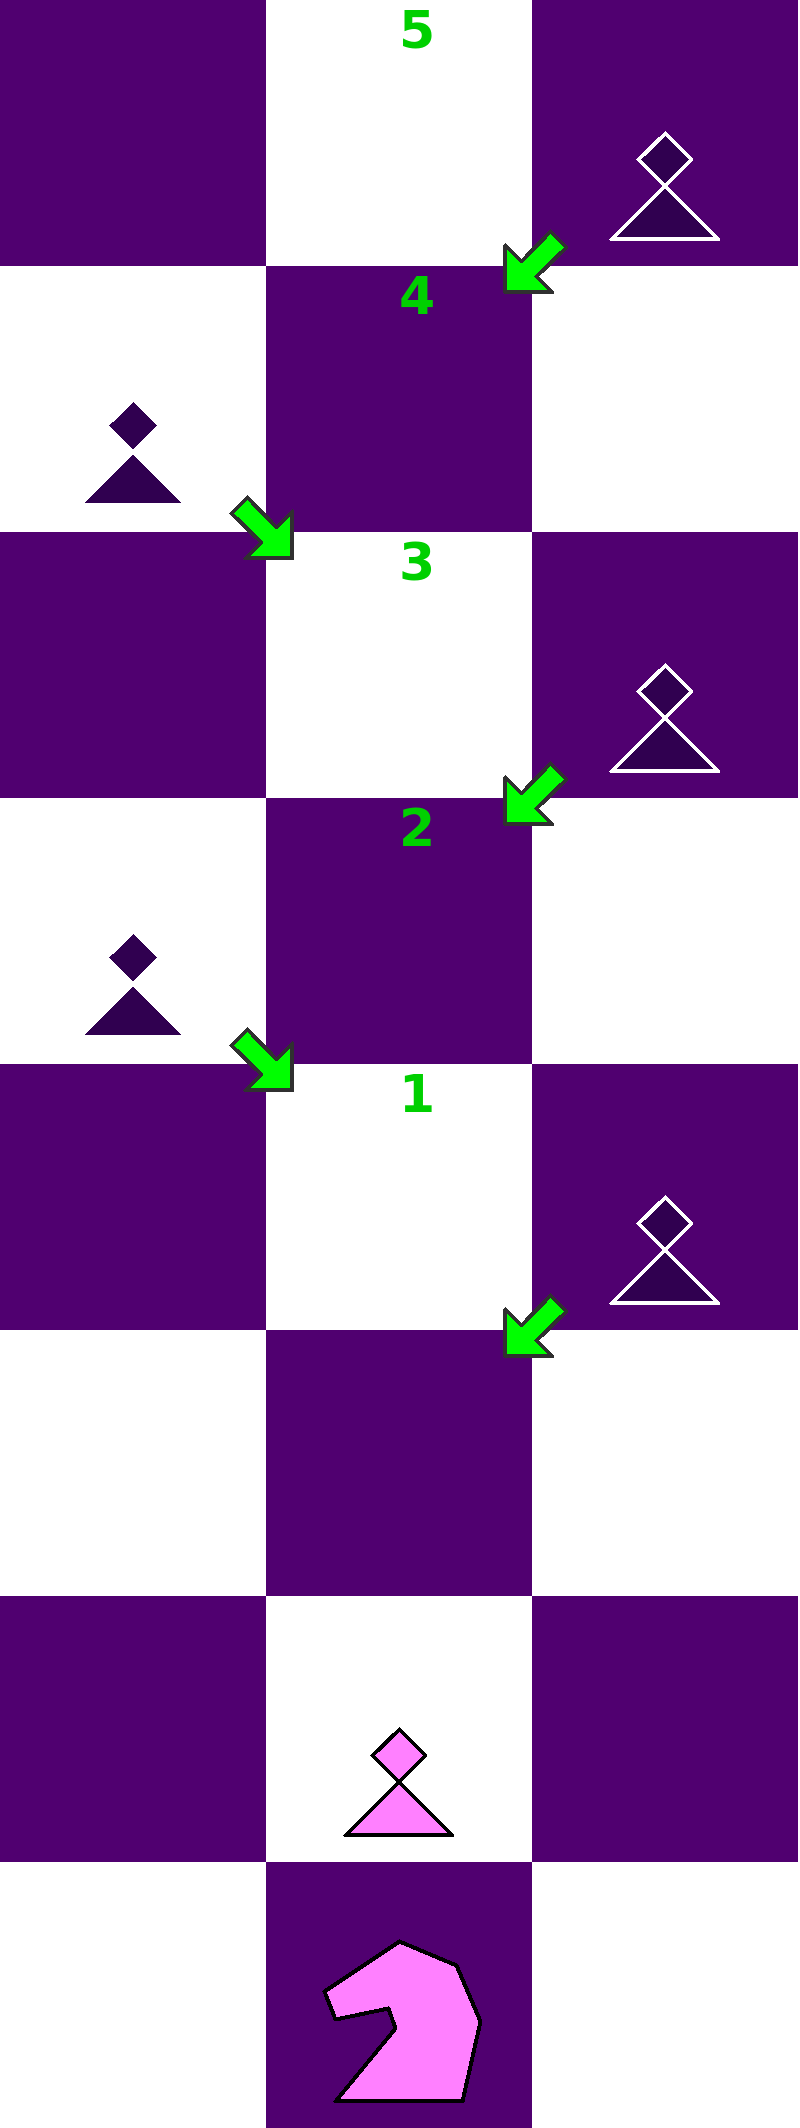
\includegraphics[width=0.1875\textwidth, keepaspectratio=true]{en_passants/10_miranda_s_veil_en_passant.png}
\caption{En passant}
\label{fig:10_miranda_s_veil_en_passant}
\end{wrapfigure}
Rush and en passant are identical to those in Classic Chess, only difference
is that Pawn can now move longer on initial turn, up to 6 fields in this
variant.

% \clearpage % ..........................................................

\vspace*{9.0\baselineskip}
\section*{Promotion}
\addcontentsline{toc}{section}{Promotion}

Promotion is non enforced, delayed variety, i.e. it's the same as in
\hyperref[sec:Age of Aquarius/Promotion]{previous chess variant}, Age of Aquarius.

\clearpage % ..........................................................

\section*{Castling}
\addcontentsline{toc}{section}{Castling}

Castling is the same as in Classical Chess, only difference is that King can move between 2 and 6 fields across.
All other constraints from Classical Chess still applies.

\noindent
\begin{figure}[!h]
% \begin{figure}[!t]
\includegraphics[width=1.0\textwidth, keepaspectratio=true]{castlings/10_mv/miranda_s_veil_castling.png}
\caption{Castling}
\label{fig:miranda_s_veil_castling}
% \centering
\end{figure}

In example above, all valid King's castling moves are numbered.

\noindent
\begin{figure}[!h]
% \begin{figure}[!t]
\includegraphics[width=1.0\textwidth, keepaspectratio=true]{castlings/10_mv/miranda_s_veil_castling_right_05.png}
\caption{Castling long right}
\label{fig:miranda_s_veil_castling_right_05}
% \centering
\end{figure}

In this example King was castling long to the right. Initial King's position is marked with "K".
After castling is finished, right Rook ends up at field immediately left to the King.

\clearpage % ..........................................................

\section*{Initial setup}
\addcontentsline{toc}{section}{Initial setup}

Compared to initial setup of Age of Aquarius, Wave is inserted between Knight and Unicorn
symmetrically, on both sides of chessboard. This can be seen in the image below:

\noindent
% \begin{figure}[t]
\begin{figure}[h]
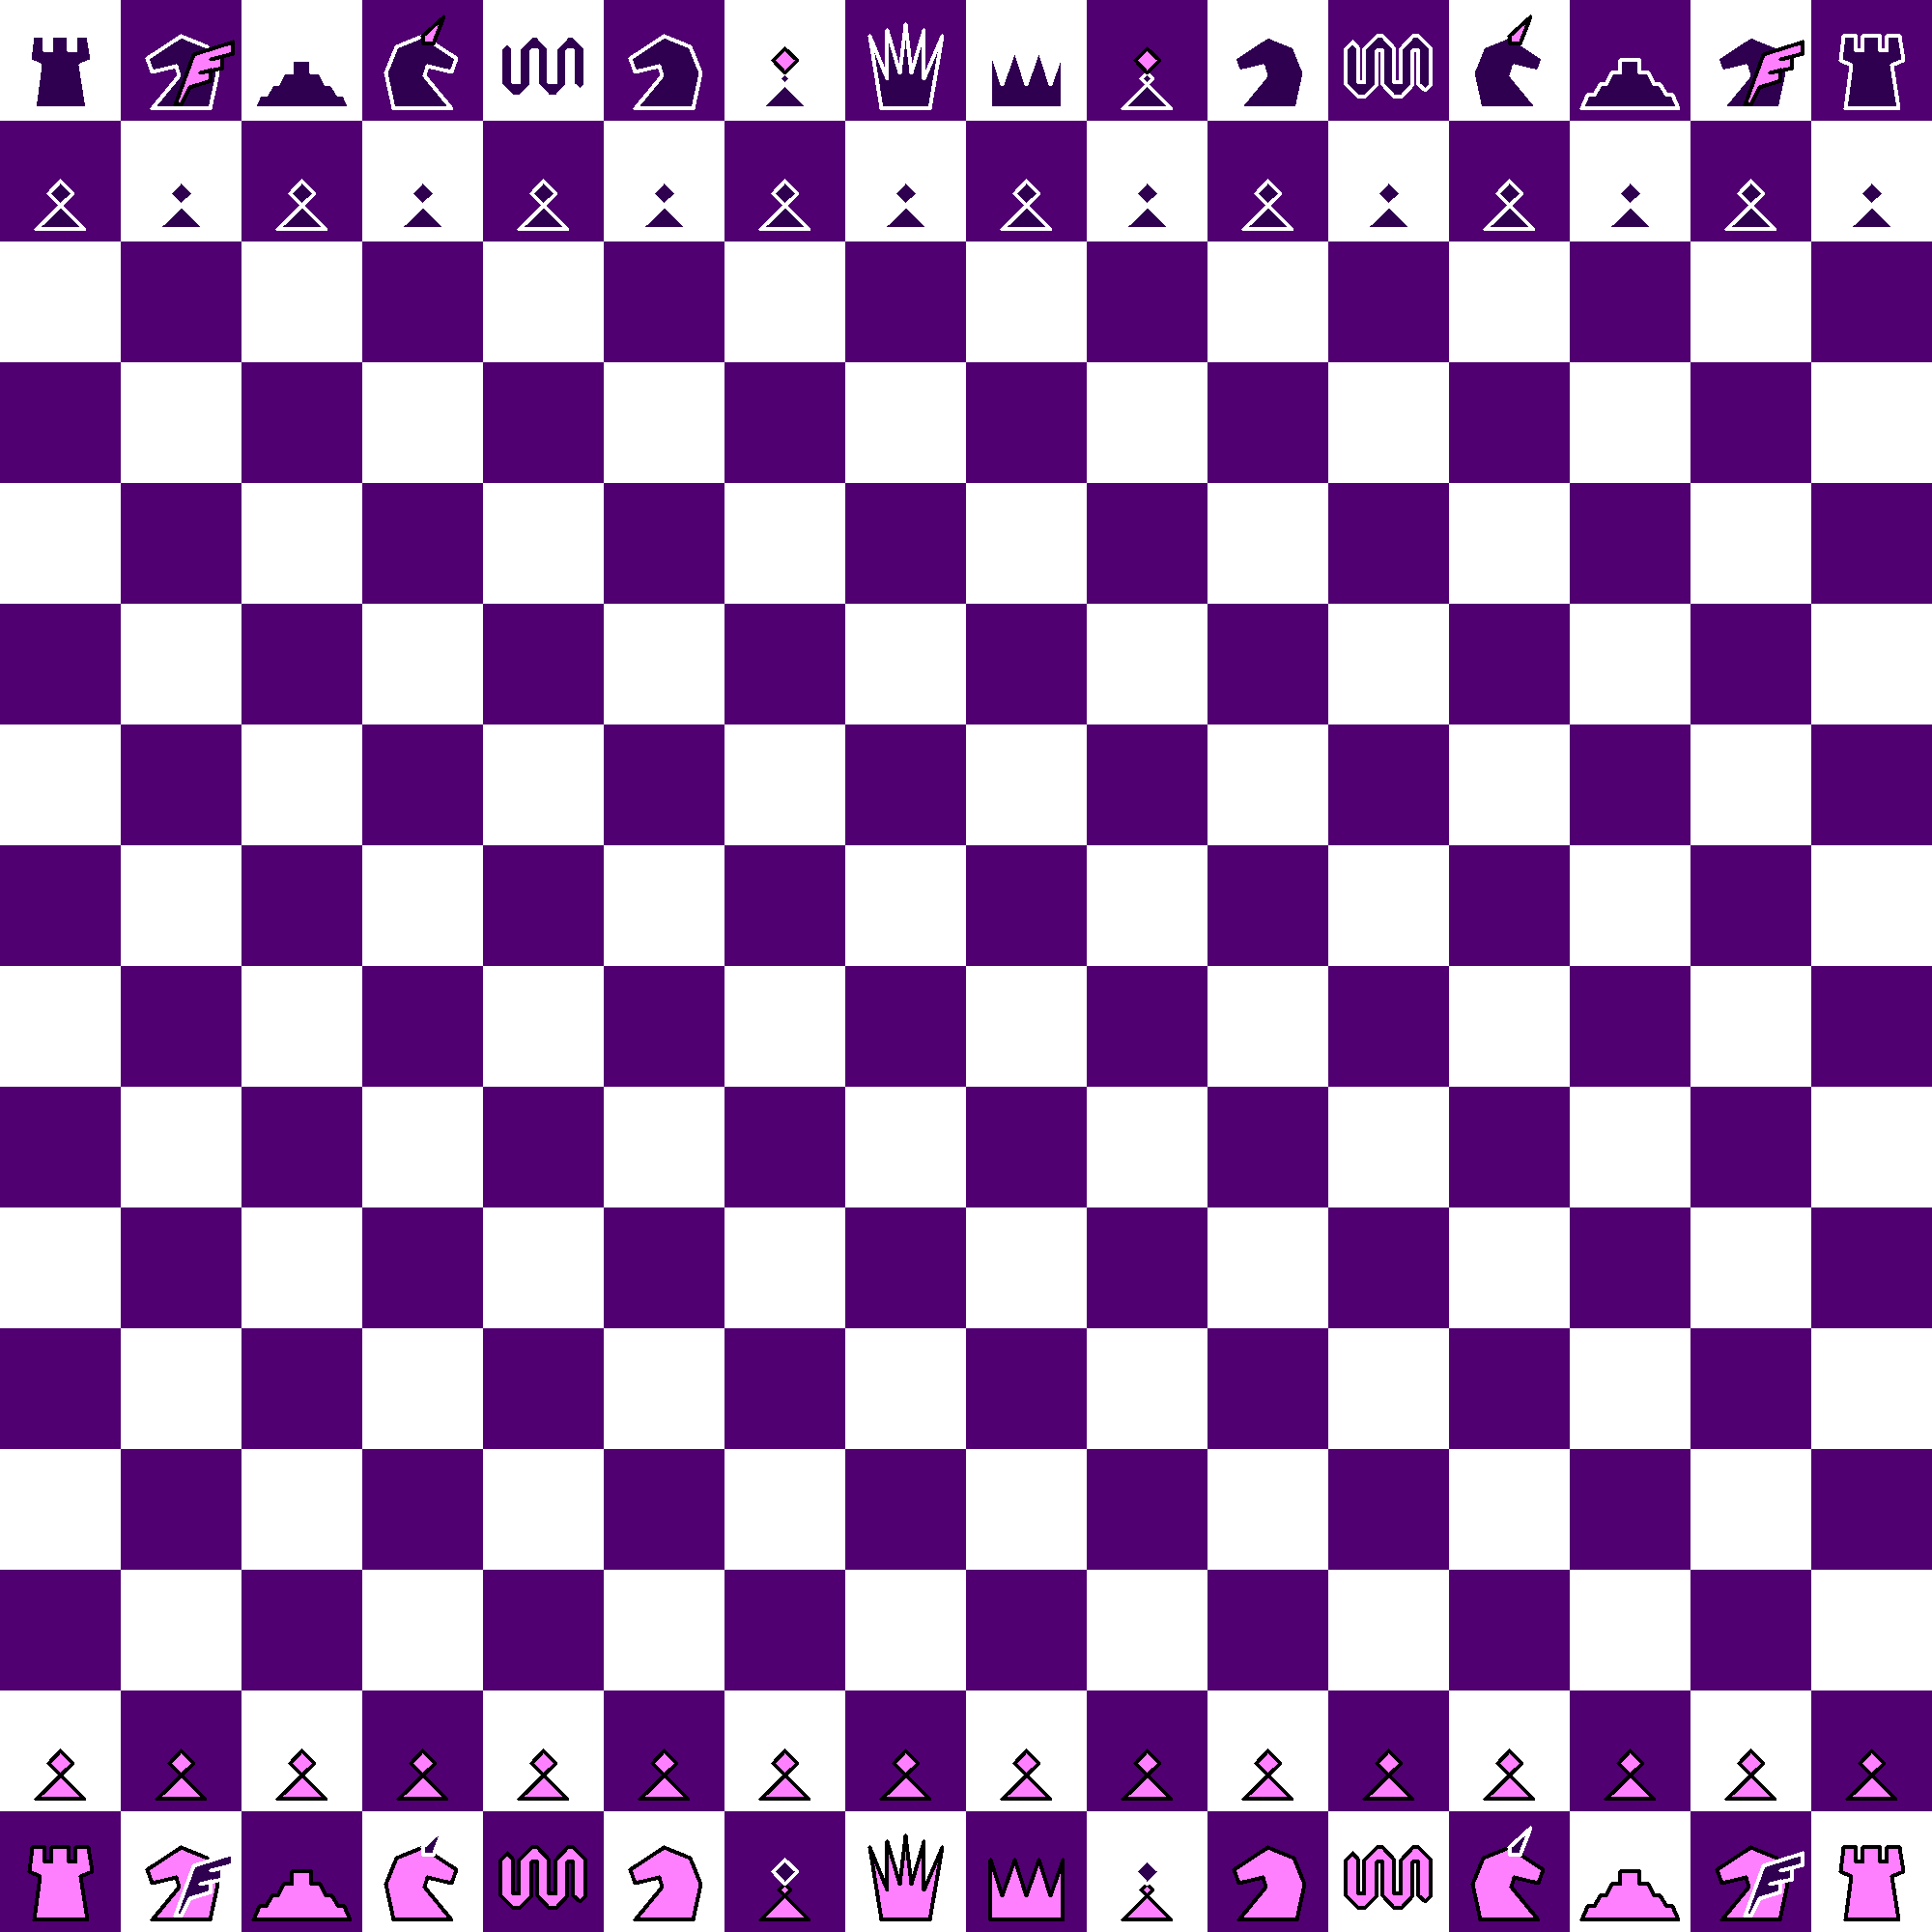
\includegraphics[width=1.0\textwidth, keepaspectratio=true]{boards/10_miranda_s_veil.png}
\caption{Miranda's veil board}
\label{fig:10_miranda_s_veil}
% \centering
\end{figure}

\clearpage % ..........................................................
% ============================================== Miranda's veil chapter
